\hypertarget{markten}{%
\chapter{Markten}\label{markten}}

\vspace{-2em}
\begin{blockquotebox}
    In een markteconomie, een sociaal systeem gebaseerd op arbeidsdeling\index{arbeidsdeling} en privaat eigendom van productiemiddelen, handelt iedereen uit eigenbelang. Dit eigenbelang dient echter tegelijkertijd de behoeften van anderen. Zo dient ieders handelen zijn medemens, terwijl hij ook door anderen gediend wordt. In dit systeem fungeert iedereen zowel als middel voor de doelen van anderen, als ook als een doel op zichzelf, strevend naar persoonlijke doelstellingen.
\footnotemark
    \par\raggedleft--- Ludwig von Mises\index{Ludwig von Mises}
\end{blockquotebox}
\footautocite{123}

Geld maakt specialisatie en arbeidsdeling\index{arbeidsdeling} mogelijk, wat het ontstaan en de groei van een markteconomie bevordert. \textbf{Een markteconomie is een sociale orde waarin mensen in staat zijn om in zeer grote aantallen samen te werken aan economische productie\index{productie}, waarbij ze elkaar vrijwillig goederen en diensten leveren voor alle betrokkenen, zonder dat een dwingende autoriteit hun handelen dicteert en coördineert.}

Om de enorme voordelen van een markteconomie te waarderen, is het goed je de impact op je leven, overlevingskansen en de kwantiteit en kwaliteit van je tijd voor te stellen wanneer je afgezonderd van de wereld of in een kleine stam zou leven, zonder ruilhandel\index{ruilhandel} met de rest van de wereld. Het aanbod van goederen zou heel klein zijn en de mogelijkheden om jezelf tegen de natuur te beschermen zouden heel beperkt zijn. Je specialiseren in bijvoorbeeld lassen of schilderen zou onmogelijk zijn, omdat je al je uren zou besteden aan het de meest basale taken die nodig zijn om niet te verhongeren of dood te vriezen. De mens wil deelnemen aan de markteconomie vanwege dwingende en ongeëvenaarde voordelen die het de deelnemers biedt, in tegenstelling tot de uitzichtloze alternatieven.

In een markteconomie hoeven individuen niet na te denken over hun eigen productie\index{productie} voor hun eigen consumptiebehoeften. Door de toenemende specialisatie en arbeidsdeling\index{arbeidsdeling} kan elk individu zich richten op de productiemethoden die hem in geld uitgedrukt de beste beloning voor zijn inspanning bieden, waardoor hij de goederen die hij voor zijn eigen behoeften aanschaft kan maximaliseren. In plaats van voor zichzelf de goederen te produceren die hij nodig heeft, specialiseert een deelnemer aan de markteconomie zich in het leveren van de goederen die hij het beste kan produceren voor anderen, en is hij afhankelijk van andere mensen voor het verkrijgen van de goederen die hij zelf nodig heeft. Uiteindelijk zorgt het kapitalistische marktsysteem ervoor dat mensen zich specialiseren in wat ze het beste kunnen en zich richten op hoe ze anderen waarde kunnen bieden, in plaats van zich te richten op wat ze zelf belangrijk vinden. Mensen kiezen in een kapitalistisch systeem om anderen te dienen, omdat het veel productiever en efficiënter is dan alleen voor jezelf, losstaand van de arbeidsdeling\index{arbeidsdeling}, te werken.

Het wonder van de markteconomie, dat vaak onderschat wordt, is de manier waarop het samenwerking tussen mensen mogelijk maakt zonder dwang, centrale regie of sociale verplichtingen. Wat de activiteiten van producenten binnen de arbeidsdeling\index{arbeidsdeling} coördineert, is hun vermogen om economische berekeningen uit te voeren over het optimale gebruik van hun middelen. Dit doen ze met behulp van een gemeenschappelijke maatstaf, namelijk de monetaire prijs, oftewel de prijs\index{prijs} uitgedrukt in geld. Naarmate een economie groeit tot een niveau waarop alle economische goederen op een markt kunnen worden gekocht en verkocht in ruil\index{ruil} voor één ander goed, kunnen deelnemers aan de economie de verschillende kosten en baten van elke handelswijze berekenen en vergelijken met hun eigen voorkeuren en met de beschikbare alternatieven. De vrijheid die iedereen heeft om zijn voorkeuren uit te drukken door middel van economisch\index{economisch} handelen, geeft iedereen de zelfzuchtige prikkel om te handelen op een manier die aan de behoeften van anderen voldoet. Het is geen autoriteit of geweld dat het handelen van mensen bepaalt, maar hun verlangen om aan hun eigen behoeften te voldoen, volgens de berekeningen die ze uitvoeren op basis van prijzen die de voorkeuren van andere deelnemers aan de markt uitdrukken. Zoals Mises het stelde:

\clearpage

\begin{blockquotebox}
    Markthandel en monetaire calculatie zijn onlosmakelijk met elkaar verbonden. Een markt waarin alleen directe ruilhandel\index{ruilhandel} plaatsvindt, is slechts een denkbeeldig idee. Aan de andere kant worden geld en monetaire calculatie bepaald door het bestaan van de markt.\footnotemark 
\end{blockquotebox}
\footautocite{124}

Wanneer de marktprijs van alle goederen wordt gemeten ten opzichte van één goed, kunnen we individuele prijzen vergelijken, zowel met andere prijzen als met hun eigen subjectieve waarderingen, en vervolgens consumptie\index{consumptie}- en productiebeslissingen nemen. Zoals al besproken in het eerste hoofdstuk van het boek, is waarde subjectief. Het kan niet objectief gemeten worden, omdat er geen constante eenheid bestaat waartegen het gemeten kan worden. Maar wanneer een individu op een markt zijn eigen keuzes maakt, weegt hij economische keuzes af tegen zijn subjectieve waarderingen. De waarden zijn misschien niet meetbaar met een constante eenheid, maar ze zijn wel vergelijkbaar met één constant referentiekader: het individu dat de waardering maakt. Door zijn eigen voorkeuren te kennen, kan de mens de verschillende voorkeuren ordenen. Hoewel we geen kardinale, numerieke waarderingen kunnen toekennen aan verschillende opties, kunnen we ze wel rangschikken op basis van onze eigen voorkeur. In dit hoofdstuk wordt een wiskundig grafisch model uitgewerkt om na te denken over hoe deze beslissingen worden genomen in de context van een markteconomie.

\vspace{-1em}
\hypertarget{markten-voor-consumentengoederen}{%
\section{Markten voor consumentengoederen}\label{markten-voor-consumentengoederen}}


Deelnemers aan een economie kopen consumptiegoederen\index{consumptiegoed} om aan hun behoeften en wensen te voldoen en ze betalen er een prijs\index{prijs} in geld voor. Individuen voeren economische berekeningen uit om de marktprijs van goederen af te wegen tegen de waardering die ze persoonlijk aan deze goederen geven. Als de prijzen veranderen, verandert natuurlijk ook de hoeveelheid van een goed dat ze kopen. Waardering is subjectief en ordinaal, niet kardinaal. Met andere woorden, individuen waarderen goederen door ze te rangschikken ten opzichte van andere goederen. Mensen hechten geen numerieke waarde aan objecten, maar vergelijken hun nut en rangschikken ze naar eigen voorkeur, zoals blijkt uit de marktkeuzes die ze maken.

We kunnen deze economische keuze zien als iets dat bereikt wordt door individuen die een waardeschaal maken: een rangorde van goederen naar individuele voorkeur. Voor elk goed weerspiegelt de waardeschaal dus de waardering van bepaalde hoeveelheden van het goed in vergelijking met monetaire eenheden.

Neem bijvoorbeeld een man die nadenkt over zijn dagelijkse behoefte aan rundvlees. Het eerste pond rundvlees van de dag, is voor hem extreem waardevol. Hij is bereid om een aanzienlijke prijs\index{prijs} te betalen om er zeker van te zijn dat hij het kan krijgen, om niet ondervoed en hongerig te zijn. Zijn inkomen, rijkdom en voorkeuren voor rundvlees in acht nemende, is hij niet bereid om \$31 betalen voor een pond rundvlees. Maar hij is wel bereid om \$30 te betalen voor het eerste pond rundvlees van de dag, wat betekent dat hij meer waarde hecht aan het eerste pond rundvlees dan aan \$30. Zodra hij dat pond heeft gekocht, wordt het tweede pond rundvlees hem iets minder waard en het overgebleven geld wordt waardevoller, omdat het minder is geworden door al voor één pond te betalen. Op dat moment is hij bereid om tot \$16 te betalen voor het tweede pond rundvlees, omdat hij het iets meer waardeert dan dit bedrag. Bij de overweging om een derde pond rundvlees te kopen, zou hij de kosten alleen dragen als de prijs \$12 of minder is. En het vierde pond zou hij alleen kopen als de prijs \$8 of lager is. Als de prijs daalt, vraagt hij meer stukken vlees, en bij een gangbare marktprijs van \$4 zou hij zijn vijfde pond rundvlees per dag consumeren. Als de prijs van rundvlees \$2 is, consumeert hij 6 pond op een dag. Bij een prijs van \$1 consumeert hij 7 pond per dag. Bij een prijs van \$0, in een wereld waarin hem gratis onbeperkt rundvlees wordt aangeboden, consumeert de man acht pond rundvlees per dag.

Op basis van deze subjectieve beslissingen kan de man zijn waardering voor verschillende hoeveelheden rundvlees en dollars rangschikken:

\begin{figure}[H]
\centering
    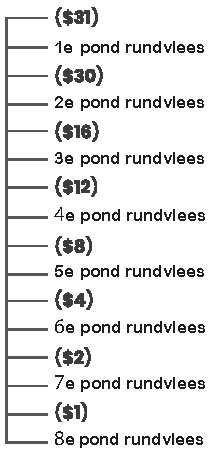
\includegraphics[height=7cm]{figures/fig20.pdf}
    \caption[Ordinale waardeschaal van consument]{Ordinale waardeschaal van consument}
    \label{fig19}
\end{figure}

De ordinale rangorde van goederen is een conceptueel hulpmiddel dat economen gebruiken om het denkproces te begrijpen dat gepaard gaat met het nemen van aankoopbeslissingen. De ordinale waardeschaal kan worden gezien als de onbewuste basis van die keuze, maar in de echte wereld wordt de koper slechts geconfronteerd met één prijs\index{prijs} en beslist hij welke hoeveelheid hij tegen die prijs\index{prijs} zal kopen. We kunnen de hoeveelheden afleiden die hij voor elke prijs\index{prijs} zou kopen. Uit deze ordinale rangschikking van rundvlees ten opzichte van monetaire eenheden, verkrijgen we een \textbf{vraagschema}: \textbf{een tabel die de gewenste hoeveelheid weergeeft bij elk prijsniveau.}

\begin{table}[!htb]
\centering
\begin{tabular}{|c|c|}  % Add vertical lines
\hline  % Top horizontal line
    \cellcolor{gray!25}Marktprijs (USD) &
    \cellcolor{gray!25}Gevraagde hoeveelheid rundvlees (pond)\\
\hline  % Horizontal line after the header
 %
 \$31 & 0 \\ \hline
 \$30 & 1 \\ \hline
 \$20 & 1 \\ \hline
 \$16 & 2 \\ \hline
 \$12 & 3 \\ \hline
 \$8 & 4 \\ \hline
 \$4 & 5 \\ \hline
 \$2 & 6 \\ \hline
 \$1 & 7 \\ \hline
 \$0 & 8 \\ \hline  % Bottom horizontal line
\end{tabular}
\caption{Consumentenvraagschema}
\label{tab3}
\end{table}

Dit vraagschema kan vervolgens grafisch worden weergegeven om de gevraagde hoeveelheden op elk prijsniveau te visualiseren. In de economie is het gebruikelijk dat de hoeveelheid op de x-as wordt uitgezet en de prijs\index{prijs} op de y-as. Dit lijkt voor iemand die uit de natuurwetenschappen komt contra-intuïtief, omdat het daar gebruikelijk is dat de afhankelijke variabele op de y-as wordt geplaatst, terwijl de onafhankelijke variabele op de x-as wordt geplaatst. In de economie is de gevraagde hoeveelheid echter een functie van de prijs\index{prijs}.

\begin{figure}[H]
\centering
    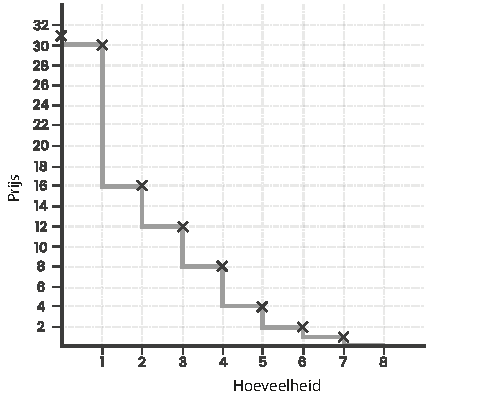
\includegraphics[width=0.7\textwidth]{figures/fig21.pdf}
    \caption[Vraagcurve]{Vraagcurve}
    \label{fig21}
\end{figure}

Zoals uitgelegd in Hoofdstuk 2 waarderen individuen de eerste eenheid van een goed meer dan alle volgende eenheden, en de waardering neemt af naarmate ze meer eenheden aanschaffen. Aan de andere kant zorgt het uitgeven van geld aan eenheden ervoor dat het kassaldo van de koper daalt, waardoor het marginale nut van geld stijgt. Met elke extra eenheid van het goed daalt de marginale prijs\index{prijs} die de koper zou betalen. Dit wijst op \textbf{de wet van de vraag}: \textbf{als de prijs\index{prijs} stijgt, daalt de gevraagde hoeveelheid. Vraagcurves hellen altijd naar beneden, of zijn verticaal, maar ze kunnen niet naar boven buigen, omdat de gevraagde hoeveelheid van een goed niet kan toenemen als de prijs\index{prijs} stijgt.}

Deze analyse is uitgevoerd voor één individu, maar kan worden toegepast op alle individuen in een markt voor een bepaald goed. Door de gevraagde hoeveelheden voor elke persoon bij elk prijspunt op te tellen, krijgen we een curve die de totale marktvraag\index{marktvraag} op een bepaald punt weergeeft. Laten we voor het gemak aannemen dat deze markt bestaat uit 100 consumenten waarvan het gemiddelde wordt vertegenwoordigd door de consument die hierboven is besproken, zodat de gevraagde hoeveelheid 100 keer zo groot is als de waarden in het individuele vraagschema. Omdat de aantallen toenemen en individuele voorkeuren lichtelijk variëren, krijgen we ook een korrelverdeling van hoeveelheden, in plaats van de stapsgewijze functie van de individuele vraagcurve die hierboven is weergegeven.

\begin{table}[H]
\centering
\begin{tabular}{|c|c|}  % Add vertical lines
\hline  % Top horizontal line
    \cellcolor{gray!25}Marktprijs (USD) &
    \cellcolor{gray!25}Gevraagde hoeveelheid rundvlees (pond) \\
\hline  % Horizontal line after the header
 %
 \$31 & 0 \\ \hline
 \$30 & 100 \\ \hline
 \$20 & 170 \\ \hline
 \$16 & 200 \\ \hline
 \$12 & 300 \\ \hline
 \$8 & 400 \\ \hline
 \$4 & 500 \\ \hline
 \$2 & 600 \\ \hline
 \$1 & 700 \\ \hline
 \$0 & 800 \\ \hline  % Bottom horizontal line
\end{tabular}
\caption{Schema van de marktvraag\index{marktvraag}}
\label{tab4}
\end{table}

\begin{figure}[H]
\centering
    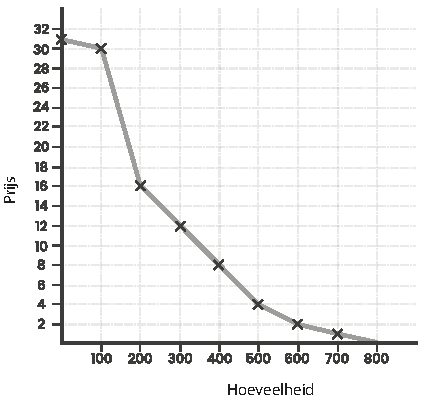
\includegraphics[width=0.7\textwidth]{figures/fig22.pdf}
    \caption[Curve van de marktvraag]{Curve van de marktvraag}
    \label{fig22}
\end{figure}

Aan de aanbodszijde voeren producenten een soortgelijke berekening uit met de goederen die ze verkopen. De persoonlijke voorkeuren van producenten kunnen worden uitgedrukt als een waardeschaal die resulteert in een rangorde van hoeveelheden van het goed ten opzichte van verschillende hoeveelheden geld. In een markteconomie waarin producenten produceren om te verkopen en niet voor hun eigen consumptie\index{consumptie}, zijn de productiekosten de hoofdfactor van de ordinale waardeschaal. Hoe hoger de marktprijs, hoe hoger de verwachte opbrengst van de verkoop en hoe meer middelen kunnen worden besteed aan de productie\index{productie} van meer eenheden van het eindproduct.

Neem als voorbeeld een slager die rundvlees verkoopt aan de voorgenoemde consumenten. Bij een prijs\index{prijs} van \$0 of \$1 per pond zal de slager geen rundvlees verkopen, omdat de prijs\index{prijs} de kosten voor het leveren van het rundvlees niet dekt. Alleen bij een prijs\index{prijs} van \$2 per pond is de slager in staat om te beginnen met produceren en kan hij 10 pond rundvlees leveren. Dit betreft een kleine hoeveelheid die hij kan leveren met een basisinstallatie die hij zich kan veroorloven om tegen die lage prijs\index{prijs} te werken door rundvlees te kopen van de dichtstbijzijnde boerderijen. Bij een prijs\index{prijs} van \$3 per pond kan hij een arbeider inhuren en 30 pond rundvlees leveren. Als hij een prijs\index{prijs} van \$4 per pond rundvlees kan verwachten, kan hij nog een arbeider inhuren en 50 pond leveren. Bij een prijs\index{prijs} van \$5 kan hij 60 pond rundvlees leveren en bij \$6 kan hij 70 pond rundvlees leveren, wat zijn maximale productie is. Verdere prijsstijgingen kunnen zijn capaciteit niet verder verhogen.

\begin{figure}[H]
\centering
    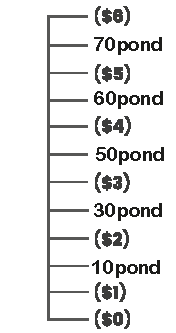
\includegraphics[height=7cm]{figures/fig23.pdf}
    \caption[Ordinale waardeschaal van de producent]{Ordinale waardeschaal van de producent}
    \label{fig23}
\end{figure}

Deze waardeschaal kan ook worden omgezet in een aanbodschema en -curve, die de hoeveelheid tonen die de producent bij elk prijsniveau levert.

\begin{table}[H]
\centering
\begin{tabular}{|c|c|}  % Add vertical lines
\hline  % Top horizontal line
    \cellcolor{gray!25}Marktprijs (USD) &
    \cellcolor{gray!25}Aangeboden hoeveelheid (in pond) \\
\hline  % Horizontal line after the header
 %
 \$7 & 70 \\ \hline
 \$6 & 70 \\ \hline
 \$5 & 60 \\ \hline
 \$4 & 50 \\ \hline
 \$3 & 30 \\ \hline
 \$2 & 10 \\ \hline
 \$1 & 0  \\ \hline
 \$0 & 0  \\ \hline  % Bottom horizontal line
\end{tabular}
\caption{Aanbodschema van de producent}
\label{tab5}
\end{table}

\begin{figure}[H]
\centering
    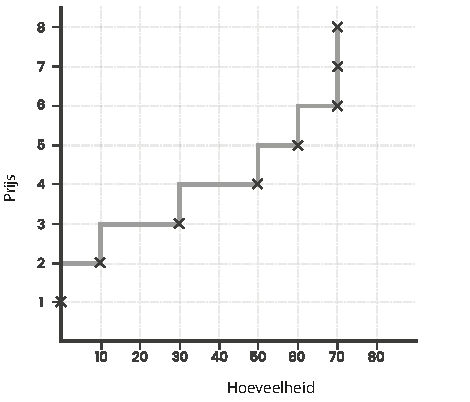
\includegraphics[width=0.7\textwidth]{figures/fig24.pdf}
    \caption[Aanbodcurve van de producent]{Aanbodcurve van de producent}
    \label{fig24}
\end{figure}

\textbf{De wet van het aanbod stelt dat naarmate de prijs\index{prijs} stijgt, de eigenaars van een economisch\index{economisch} goed meer bereid en in staat zijn om grotere hoeveelheden te verkopen. Als gevolg hiervan hellen aanbodcurves alleen omhoog.} Dit kun je begrijpen door te kijken naar de voorkeur van individuen om goederen te bezitten, welke afneemt naarmate de prijs\index{prijs} die ze voor hun goederen kunnen krijgen toeneemt. Voor producenten op de markt kan men ook inzien dat hogere prijzen de stimulans vergroten om meer te gaan produceren en grotere investeringen mogelijk maken om meer grondstoffen en arbeiders te verwerven, wat resulteert in grotere geleverde hoeveelheden.

Voor een goed met meerdere producenten kunnen de aanbodschema\textquotesingle s en -curves van alle producenten worden samengevoegd tot één marktaanbodcurve. De marktaanbodcurve toont de hoeveelheid die door alle producenten van het goed zal worden geproduceerd bij elk gegeven prijsniveau. Laten we voor dit voorbeeld aannemen dat er tien producenten zijn en dat het bovenstaande voorbeeld hun gemiddelde weergeeft.

\begin{table}[H]
\centering
\begin{tabular}{|c|c|}  % Add vertical lines
\hline  % Top horizontal line
    \cellcolor{gray!25}Marktprijs (USD) &
    \cellcolor{gray!25}Aangeboden hoeveelheid (pond) \\
\hline  % Horizontal line after the header
 %
 \$7 & 700 \\ \hline
 \$6 & 700 \\ \hline
 \$5 & 600 \\ \hline
 \$4 & 500 \\ \hline
 \$3 & 300 \\ \hline
 \$2 & 100 \\ \hline
 \$1 & 0  \\ \hline
 \$0 & 0  \\ \hline  % Bottom horizontal line
\end{tabular}
\caption{Aanbodschema van de markt}
\label{tab6}
\end{table}

\begin{figure}[H]
\centering
    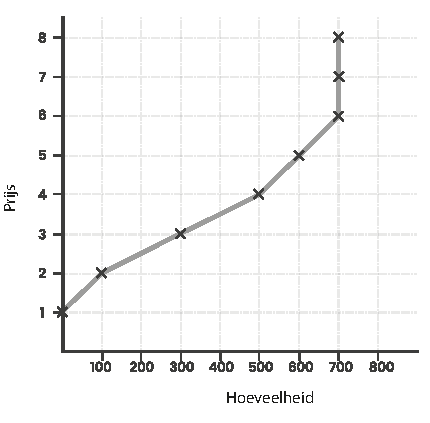
\includegraphics[width=0.7\textwidth]{figures/fig25.pdf}
    \caption[Aanbodcurve van de markt]{Aanbodcurve van de markt}
    \label{fig25}
\end{figure}

\clearpage
\hypertarget{evenwicht}{%
\section{Evenwicht}\label{evenwicht}}

Bij een prijs\index{prijs} van nul is de gevraagde hoeveelheid zeer groot, terwijl de geleverde hoeveelheid waarschijnlijk nul is. Als de prijs\index{prijs} vanaf nul stijgt, neemt de gevraagde hoeveelheid af, terwijl de geleverde hoeveelheid toeneemt. Er is maximaal één prijspunt waarbij de gevraagde en geleverde hoeveelheden gelijk zijn, en dat wordt de \textbf{evenwichtsprijs} genoemd. Dit prijspunt werkt als een magneet op kopers en verkopers en trekt hen aan om hier altijd rond te handelen.

Als de prijs\index{prijs} hoger is dan de evenwichtsprijs, leveren de verkopers een grotere hoeveelheid van het goed dan de kopers vragen, wat resulteert in een \textbf{overschot}. Verkopers zouden de prijs\index{prijs} natuurlijk willen verlagen om meer kopers aan te moedigen hun overtollige goederen te kopen, waardoor de prijs\index{prijs} naar de evenwichtsprijs daalt. Als de prijzen daarentegen lager zijn dan de evenwichtsprijs, dan vragen de consumenten een grotere hoeveelheid dan de verkopers leveren, wat leidt tot een \textbf{tekort.} Dit zou verkopers vervolgens stimuleren om hun prijzen te verhogen om het aanbod te rantsoeneren en hun winst te maximaliseren. Ze kunnen hun prijzen blijven verhogen tot de evenwichtsprijs is bereikt, waarna verdere prijsverhogingen zouden leiden tot minder kopers en een overschot. De dynamiek van de markt zal de prijs\index{prijs} altijd naar de evenwichtsprijs leiden.

We zien het marktevenwicht uit het vorige voorbeeld door de vraag- en aanbodcurves op één grafiek te leggen. Omdat de vraagcurve naar beneden helt, terwijl de aanbodcurve alleen maar stijgt, kunnen de twee curves elkaar slechts op één punt snijden, als ze elkaar al doorkruisen. In deze markt zouden de tien producenten van rundvlees 500 pond rundvlees produceren om te verkopen tegen een prijs\index{prijs} van \$4, en de 100 consumenten zouden dit allemaal kopen tegen een prijs\index{prijs} van \$4. Er zijn geen overschotten of tekorten. Als er veranderingen optreden in de waardeschalen van de individuen, zullen de vraag- en aanbodcurves zich aanpassen om deze veranderingen te weerspiegelen en zal het evenwicht verschuiven, maar het zal kopers en verkopers blijven aantrekken.

\begin{figure}
\centering
    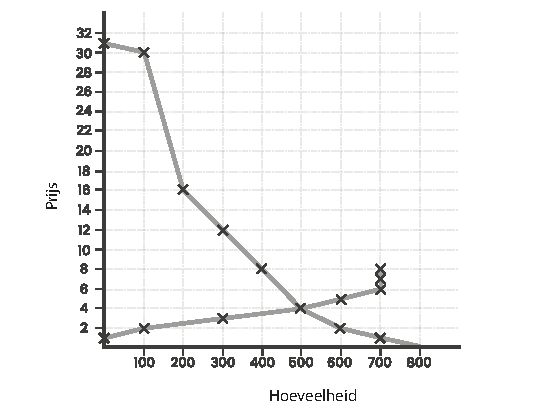
\includegraphics[width=0.8\textwidth]{figures/fig26.pdf}
    \caption[Marktevenwicht]{Marktevenwicht}
    \label{fig26}
\end{figure}

Alle deelnemers aan de markt handelen op manieren die in hun eigen voordeel zijn. Ze stemmen ermee in om aan deze transacties deel te nemen, omdat ze verwachten er voordeel uit te halen, en ze kiezen aan welke transacties ze deelnemen, omdat ze denken dat ze de best mogelijke deal krijgen. Het concept van evenwicht helpt om te begrijpen hoe vrijwillige marktinteracties tot prijzen komen zonder dwingende autoriteit of opgelegd besluit. Toch is het beter om markten\index{markten} te zien als evenwichtsprocessen dan je in te beelden dat markten\index{markten} tot starre evenwichtsprijzen voor alle goederen leiden. De wereld van menselijk handelen\index{menselijk handelen} verandert voortdurend en de voorwaarden van vraag en aanbod worden voortdurend beïnvloed door diverse factoren. Naarmate hun eigen individuele omstandigheden veranderen, verandert ook de realiteit van de markt. Evenwicht is dus geen eindtoestand die markten\index{markten} bereiken. In plaats daarvan zijn markten\index{markten} voortdurende ontdekkingsprocessen waarbij vraag en aanbod zich altijd uitbalanceren naar prijzen die de meeste waarde voor de betrokken deelnemers opleveren.

Prijsschommelingen veranderen de omvang van wat een individu vraagt, grafisch uitgedrukt in de vraagcurves. Maar veranderingen in andere factoren die betrekking hebben op de vraag leiden tot een herformulering van de relatie tussen prijs\index{prijs} en vraag, met een nieuwe gevraagde hoeveelheid voor elke prijs\index{prijs}, en dus een verschuiving in de hele vraagcurve. Enkele factoren die de vraagcurve kunnen verschuiven zijn veranderende voorkeuren, veranderingen in inkomen en welvaart, of veranderende prijzen van andere goederen en diensten. Als het inkomen of de welvaart van de koper toeneemt, zal hij waarschijnlijk meer van de meeste goederen vragen en zal de vraagcurve naar rechts verschuiven, waardoor de gevraagde hoeveelheid bij alle prijsniveaus toeneemt. Maar voor minderwaardige goederen zou een stijging van het inkomen of de rijkdom het tegenovergestelde effect veroorzaken, waarbij de gevraagde hoeveelheid bij alle prijsniveaus afneemt en de vraagcurve naar links verschuift, omdat mensen zich betere alternatieven kunnen veroorloven. Bonen zijn een voorbeeld van zo\textquotesingle n minderwaardig goed: als de inkomens over de hele wereld stijgen, zullen mensen waarschijnlijk hun vraag naar bonen verlagen en hun vraag naar rundvlees verhogen.

De vraagcurve van een goed kan ook worden beïnvloed door veranderingen in de prijzen van andere goederen. Als de prijs\index{prijs} van een goed stijgt, daalt de gevraagde hoeveelheid en daalt de gevraagde hoeveelheid van een aanvullend goed op alle prijsniveaus, waardoor de vraagcurve naar links verschuift. Als datzelfde goed in prijs\index{prijs} daalt, zal de gevraagde hoeveelheid stijgen, terwijl de gevraagde hoeveelheid van het aanvullende goed op alle prijsniveaus zal stijgen, waardoor de vraagcurve naar rechts verschuift. Het tegenovergestelde geldt als het een vervangend goed is.

Behalve door wordt het marktaanbod ook beïnvloed door de productiekosten en de prijzen van verwante producten die met dezelfde productiefactoren kunnen worden geproduceerd. Als de productiekosten van producenten stijgen, kunnen ze lagere hoeveelheden van hun product leveren bij elk prijsniveau, waardoor de aanbodcurve naar links verschuift. Als de producent zich anderzijds realiseert dat hij meer winst kan maken door zijn productiefactoren te verschuiven naar de productie\index{productie} van een ander goed waarvan de prijs\index{prijs} stijgt, zou dat de aanbodcurve voor het oorspronkelijke goed naar links verschuiven, waardoor de geleverde hoeveelheid op alle prijsniveaus daalt.

Dit grafische raamwerk helpt te verklaren hoe een vrije markt reageert op veranderingen in vraag en aanbod in de loop van de tijd. In industrieën waar producenten door technologische innovatie steeds grotere hoeveelheden van een goed tegen een bepaalde prijs\index{prijs} kunnen produceren, resulteert dit in een verschuiving van de aanbodcurve van de markt naar rechts. Het gevolg van deze verschuiving is dat de evenwichtsprijs daalt en de verkochte hoeveelheid toeneemt. Deze trend is te zien in de hightech industrie, waar prijzen voortdurend dalen en de geproduceerde hoeveelheid toeneemt door de verhoogde productiviteit en technologische innovatie. Grafisch kan dit worden geïllustreerd met de verschuiving van S1 naar S2 in Figuur 27.

\begin{figure}[h]
\centering
    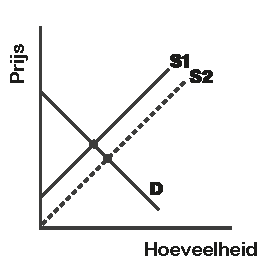
\includegraphics[]{figures/fig27.pdf}
    \caption[Verschuivingen in de aanbodcurve]{Verschuivingen in de aanbodcurve}
    \label{fig27}
\end{figure}

Als het omgekeerde zou gebeuren, en een probleem met de aanbodketen de productie\index{productie} van het goed negatief zou beïnvloeden, zouden producenten een kleinere hoeveelheid van het goed kunnen leveren bij elk gegeven prijsniveau, waardoor de aanbodcurve effectief naar links zou verschuiven. In deze situatie zou het nieuwe evenwicht met de vraagcurve ontstaan bij een hogere prijs\index{prijs} en een lagere hoeveelheid. Een natuurramp is hier een extreem voorbeeld van, waarbij de beschikbare hoeveelheden van een goed enorm afnemen, terwijl de prijzen stijgen. Dit wordt grafisch weergegeven met de verschuiving van S2 naar S1 in Figuur 27.

We kunnen dezelfde analyse toepassen op verschuivingen in de vraagcurve. Factoren die de vraag van de consument bij alle prijzen doen toenemen, zoals een toegenomen voorkeur van de consument voor het goed ongeacht de prijs\index{prijs}, of een stijging van de prijs\index{prijs} van vervangende goederen of een daling van de prijs\index{prijs} van aanvullende goederen, zouden de vraagcurve naar rechts doen verschuiven, grafisch weergegeven als de verschuiving van curve D1 naar curve D2 in Figuur 28. Een daling van de consumentenvraag naar het goed tegen alle prijzen, of een stijging van de prijs\index{prijs} van aanvullende goederen of een daling van de prijs\index{prijs} van een vervangend goed, zou de vraagcurve naar links doen verschuiven. Grafisch wordt dit weergegeven door de verschuiving van curve D2 naar D1 in Figuur 28.

\begin{figure}[h]
\centering
    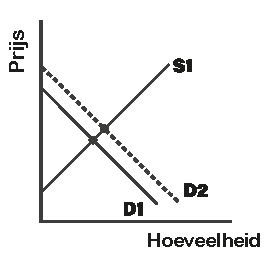
\includegraphics[]{figures/fig28.pdf}
    \caption[Verschuivingen in de vraagcurve]{Verschuivingen in de vraagcurve}
    \label{fig28}
\end{figure}

\hypertarget{markten-van-producentgoederen}{%
\section{Markten van producentgoederen}\label{markten-van-producentgoederen}}

Producenten baseren hun beslissingen ook op het nut dat verschillende handelsmethoden hun opleveren. Het verschil tussen de keuze van de consument en die van de producent ligt aan het feit dat de producent geen persoonlijk nut ontleent aan de factoren die hij gebruikt; hij gebruikt ze puur om de geldelijke winst die hij met zijn bedrijf\index{bedrijf} kan behalen te maximaliseren. Consumentensoevereiniteit betekent dat de producent al zijn zakelijke beslissingen baseert op de wensen en behoeften van de consument.

Het productieproces\index{productieproces} bestaat uit het omzetten van productiefactoren in eindgoederen en -diensten die aan consumenten worden verkocht. De hoeveelheid van elke ingezette productiefactor wordt bepaald door de kosten ervan te vergelijken met de marginale inkomsten die ze bijdraagt aan de bedrijfsactiviteiten. Elke extra eenheid arbeid of kapitaal\index{kapitaal} die in de productie\index{productie} wordt ingezet, resulteert in een marginale toename van de hoeveelheid geproduceerde eindproducten. Werkgevers zullen productiefactoren blijven inzetten zolang de verwachte marginale opbrengst van de ingezette factor hoger is dan de kosten van het inzetten ervan. De prijzen van deze productiefactoren worden op hun beurt bepaald door hoe goed ze voldoen aan de vraag van de consument. Als het inhuren van een extra arbeider voor een dag naar verwachting \$10 aan inkomsten zal toevoegen aan een bedrijf\index{bedrijf}, zal dat bedrijf\index{bedrijf} alleen een extra arbeider inhuren als de vraag naar loon minder is dan \$10 per dag. Als een ondernemer overweegt om een machine te kopen die \$1.000 kost, zal hij deze alleen kopen als de verwachte marginale verdiscontering van het product dat het gedurende zijn levensduur produceert groter is dan \$1.000. Uiteindelijk is het dus de waardering van eindproducten door de consument die waarde geeft aan productiefactoren. De functie van de ondernemer is om uitspraken te doen over de toekomstige behoeften van consumenten, te investeren in de productiefactoren voordat de productie\index{productie} plaatsvindt, en het risico\index{risico} op zich te nemen dat hij het mis heeft over wat consumenten zullen waarderen na de productie\index{productie}.

Het is zinloos om te klagen over lonen of kapitaalopbrengsten. Dit zijn cruciale signalen van de markt die individuen vertellen hoe waardevol hun arbeid, land en kapitaal\index{kapitaal} zijn. Ondernemers kunnen niet zomaar zelf de lonen bepalen; ze zijn afhankelijk van de subjectieve waarderingen van consumenten. Als een ondernemer besluit om te veel te betalen voor lonen, zal hij zijn winstgevendheid verliezen en vervangen worden door ondernemers die een gepastere prijs\index{prijs} betalen. Als de ondernemer besluit een lager loon te betalen, zal hij zijn werknemers verliezen aan anderen die bereid zijn een hogere prijs\index{prijs} te betalen. Om ondernemer te blijven in een bepaalde branche, heeft de ondernemer geen andere keuze dan werknemers te betalen voor hun marginale productiviteit. In een vrijemarktsysteem kunnen kapitalisten en ondernemers de werknemers niet onderdrukken, omdat ze vrij zijn om elders te gaan werken en omdat de consumenten hun producten elders kunnen kopen. Alleen door zorgvuldig en correct te koorddansen tussen werknemers en consumenten kunnen ondernemers in bedrijf\index{bedrijf} blijven.

\hypertarget{economisch-handelen-in-de-marktorde}{%
\section{Economisch handelen in de marktorde}\label{economisch-handelen-in-de-marktorde}}

We kunnen het marktsysteem zien als het grotere kader waarbinnen al het eerder besproken economisch\index{economisch} handelen kan plaatsvinden met de grootste toename in productiviteit. Arbeid, kapitaal\index{kapitaal}, technologie, macht, handel en geld zijn allemaal instrumenten die veel productiever kunnen worden ingezet in de context van vrije en onpersoonlijke ruilhandel\index{ruilhandel} op de markt. Als gevolg hiervan heeft de markteconomie de reële lonen van arbeiders gestaag verhoogd, omdat de markteconomie voortdurend nieuwe manieren vindt om de waarde van menselijke tijd te verhogen, door deze op de meest productieve manier te gebruiken om aan de behoeften van andere mensen te voldoen.

Marktdeelnemers communiceren hun veranderende voorkeuren en voorwaarden aan elkaar door te beslissen om tegen bepaalde prijzen wel of niet te kopen. Dit proces van wederzijdse samenwerking stelt alle marktdeelnemers in staat om in hun eigen belang te handelen, terwijl ze hun handelingen coördineren om elkaar beter van dienst te zijn. Alle voorkeuren van consumenten worden aan andere marktdeelnemers kenbaar gemaakt door hun keuzes om tegen een bepaalde prijs\index{prijs} wel of niet te kopen, waardoor producenten waardevolle kennis krijgen waarmee ze hun productiebeslissingen kunnen maken. Zoals Mises het stelde:

\begin{blockquotebox}
    Het marktproces is de aanpassing van de individuele handelingen van de verschillende marktdeelnemers aan de vereisten van onderlinge samenwerking. De marktprijzen vertellen de producenten wat ze moeten produceren, hoe ze moeten produceren en in welke hoeveelheid. De markt is het brandpunt waar de activiteiten van de individuen samenkomen.\footnotemark    
\end{blockquotebox}
\footautocite{125}

Mises voegt hier verder aan toe:

\begin{blockquotebox}
    In de natuur heersen onverzoenlijke belangenconflicten. De middelen voor levensonderhoud zijn schaars. De groei van populaties heeft de neiging om het bestaansminimum te overtreffen. Alleen de sterkste planten en dieren overleven. De vijandschap tussen een dier dat verhongert en een ander dat het voedsel wegkaapt is onverbiddelijk. Sociale samenwerking door arbeidsdeling\index{arbeidsdeling} lost zulke vijandigheid op. Het vervangt vijandigheid door samenwerking en wederkerigheid. De leden van de samenleving zijn verenigd in een gemeenschappelijke onderneming.\footnotemark    
\end{blockquotebox}
\footautocite{126}

\hypertarget{consumentensoevereiniteit}{%
\section{Consumentensoevereiniteit}\label{consumentensoevereiniteit}}

De zorgvuldige analyse van het marktproces illustreert waarom de consument in een vrije markt koning is. Individuen zijn in een markteconomie soeverein in hun hoedanigheid als consument, omdat de producenten geen manier hebben om hen te dwingen hun goederen te kopen, behalve door goederen te produceren die voldoen aan de behoeften en verlangens van de consument tegen een prijs\index{prijs} die zij zich kunnen veroorloven. Producenten investeren hun kapitaal\index{kapitaal} in het productieproces\index{productieproces} en zijn afhankelijk consumenten die hun product goed vinden, zodat hun investering niet verloren gaat. Producenten bevinden zich niet in een positie om de voorwaarden te dicteren of consumenten uit te buiten; die hebben alle keuze. Zoals Mises uitlegt:

\begin{blockquotebox}
    Als ze er niet op uit waren om op de goedkoopste markt aankopen te doen en hun productiefactoren zo in te richten dat ze op de beste en goedkoopste manier aan de vraag van de consumenten konden voldoen, dan zouden ze gedwongen worden om hun bedrijf\index{bedrijf} te stoppen. Efficiëntere mensen die er beter in slagen de productiefactoren te kopen en te verwerken, zouden hen vervangen. De consument bevindt zich in een positie waarin hij zijn opwellingen en wensen de vrije loop kan laten. De ondernemers, kapitalisten en boeren hebben geen keuze; ze zijn verplicht om zich in hun bedrijfsvoering te houden aan de wensen van het kopende publiek. Elke afwijking van de lijnen die zijn voorgeschreven door de vraag van de consumenten is voor eigen rekening. De kleinste afwijking, bewust gekozen of veroorzaakt door fouten, slecht beoordelingsvermogen of onnauwkeurigheid, beperkt hun winsten of doet ze zelfs helemaal verdwijnen. Een ernstigere afwijking resulteert in verliezen en tast zo hun vermogen aan of slokt dit volledig op. Kapitalisten, ondernemers en landeigenaren kunnen hun rijkdom alleen behouden en vergroten door de orders van consumenten zo goed mogelijk uit te voeren.\footnotemark    
\end{blockquotebox}
\footautocite{127}

Mises vergelijkt de macht van consumenten in de markt vervolgens met het democratische proces en laat zien dat het superieur is, omdat het tegemoet komt aan de behoeften van iedereen, terwijl democratie alleen tegemoet komt aan de behoeften van de winnende meerderheid:

\begin{blockquotebox}
    Met elke cent die wordt uitgegeven bepalen de consumenten de richting van alle productieprocessen en de details van de organisatie van alle bedrijfsactiviteiten. Deze stand van zaken is beschreven door de markt een democratie te noemen waarin elke cent het recht geeft om te stemmen. Het zou correcter zijn om te zeggen dat een democratische grondwet een plan is om aan de burgers in het bestuur dezelfde macht toe te kennen die de markteconomie hen geeft in hun mogelijkheden als consumenten. De vergelijking is echter niet perfect. In de politieke democratie zijn alleen de stemmen die uitgebracht worden voor de kandidaat of het plan van de meerderheid effectief om de gang van zaken vorm te geven. De stemmen van de minderheid hebben geen directe invloed op het beleid. Maar op de markt wordt geen enkele stem tevergeefs uitgebracht. Elke cent die wordt uitgegeven heeft de macht om de productieprocessen te beïnvloeden. Boekuitgevers bedienen niet alleen de meerderheid door detectives te publiceren, maar ook de minderheid die lyrische poëzie en filosofische geschriften leest. De bakkerijen bakken niet alleen brood voor gezonde mensen, maar ook voor zieken met een speciaal dieet. De beslissing van een consument wordt uitgevoerd met de volledige vaart die hij er achter zet met zijn bereidheid om een bepaald geldbedrag uit te geven.\footnotemark    
\end{blockquotebox}
\footautocite{128}

\hypertarget{een-contrast-van-benaderingen}{%
\section{Een contrast van benaderingen}\label{een-contrast-van-benaderingen}}

Al zolang er regeringen bestaan, bestaat de drang om prijzen per wet vast te stellen. Dit heeft geleid tot een hele reeks verschrikkelijke en voorspelbare gevolgen.\autocite{129} Maar de vele en diverse vergeefse pogingen van centrale overheden om prijzen vast te leggen hebben één positief gevolg gehad: ze hebben veel mensen laten inzien dat economie een product is van menselijk handelen\index{menselijk handelen}, ook al verwoorden ze het misschien niet helemaal in deze Misesiaanse bewoordingen. Door de analyse van de politicus die de prijscontrole oplegt en die van de econoom tegenover elkaar te zetten, zien we duidelijk de kracht van de economische manier van denken.

De politicus die ontevreden is over een marktprijs en deze wil veranderen, ziet de prijs\index{prijs} als iets willekeurigs dat hij kan bepalen. Hij denkt niet op een economische manier omdat hij prijzen niet ziet als het resultaat van menselijk handelen\index{menselijk handelen}, als een weerspiegeling van menselijke keuzes. Het element van individuele en persoonlijke keuze bij het bepalen van prijzen wordt genegeerd. De aandacht gaat in plaats daarvan naar de politieke en sociale implicaties van deze prijzen. Hij vergelijkt de huidige realiteit met een hypothetische realiteit waarin de prijs\index{prijs} lager is en de geconsumeerde hoeveelheid hoger, terwijl al het andere hetzelfde blijft.

De meeste politieke leiders zijn niet op hun positie gekomen door hun economische kennis. Het begrijpen van economie is wellicht een belangrijke belemmering voor succes in de politiek. Politici beschouwen de prijzen van economische goederen en diensten louter als een maatstaf voor hun betaalbaarheid en ze weten dat hoe lager de prijzen, hoe gelukkiger de bevolking. Zonder prijzen te begrijpen als het resultaat van menselijk handelen\index{menselijk handelen} in reactie op de economische realiteit, denkt de politicus dat hij prijzen kan sturen om zijn gewenste resultaten te bereiken en dus zal hij wetten aannemen die maximumprijzen voor specifieke goederen voorschrijven. De foutieve redenering gaat ervan uit dat als de prijs\index{prijs} van een goed wettelijk wordt vastgelegd, kopers en verkopers geen andere keuze hebben dan tegen die prijs\index{prijs} te kopen en te verkopen.

Als de politieke leider een econoom wil raadplegen, zal hij waarschijnlijk de voorkeur geven aan het advies van kwantitatieve economen die schijnbaar correcte argumenten voor dit beleid kunnen produceren. Een kwantitatief econoom kan het effect van prijzen op economische activiteit wiskundig modelleren en een theoretisch kwantitatief verband vinden tussen de prijs\index{prijs} van een goed, het bestedingsniveau in de economie en economische groei. Het is mogelijk om een causaal mechanisme te veronderstellen, gebaseerd op gegevens uit de echte wereld, waarbij een verlaging van de prijs\index{prijs} van een essentieel goed de levensstandaard van een groot deel van de bevolking verhoogt, wat resulteert in meer sparen, meer investeringen en een snellere economische groei. Met een kwantitatieve observatie van de grootheden en ontoetsbare aannames over de richting van causaliteit kan de kwantitatieve econoom de overheid\index{overheid} een schijnbaar wetenschappelijke formule aanreiken om de economie te verbeteren door prijzen bij wet op te leggen. Zonder een constante meeteenheid kunnen deze vergelijkingen niet nauwkeurig zijn, zodat elk gewenst resultaat kan worden geregeld.

Vanuit het perspectief van de degelijke econoom is de prijs\index{prijs} echter meer dan alleen een maatstaf voor de betaalbaarheid van een goed. Het is een product van vrijwillige menselijke handelingen en keuze en de oplossing van een calculatieprobleem voor de producent en consument. Als de overheid\index{overheid} een andere prijs\index{prijs} voor het goed oplegt, is er geen garantie dat de betrokken individuen dezelfde handelingen zullen verrichten die ze anders ook hadden verricht, noch dat ze elkaar op dezelfde manier tevreden kunnen stellen.

Prijzen zijn geen willekeurige getallen die door winkeliers worden bedacht, ze komen tot stand door een complex samenspel van mensen die handelen en vraag en aanbod op de markt beïnvloeden. Een markttransactie die plaatsvindt tegen een bepaalde prijs\index{prijs} geeft aan dat zowel de koper als de verkoper ervoor gekozen hebben om deze prijs\index{prijs} te accepteren. Beiden hadden natuurlijk liever een andere prijs\index{prijs} gezien; de koper had liever een lagere prijs\index{prijs} gezien en de verkoper had liever een hogere prijs\index{prijs} gezien, maar de huidige prijs\index{prijs} was duidelijk aanvaardbaar voor beiden, gezien het feit dat ze handel dreven. Als een politicus tussenbeide zou komen en de prijs\index{prijs} bij wet met dwang te veranderen, is er geen reden om aan te nemen dat de koper en verkoper dezelfde beslissingen zouden nemen als voorheen. En vanuit het perspectief van een econoom zou zo\textquotesingle n wet veel destructiever zijn dan de prijzen die op de markt waren ontstaan, hoe onaangenaam die ook waren voor de leiders.

Wat de marktprijs van een goed ons vertelt, is dat de verkoper tevreden is met de verkoop van dit goed voor deze prijs\index{prijs}. Als kopers weigeren dit goed voor die prijs\index{prijs} te kopen, dan moet de producent zijn prijzen verlagen. Als hij zijn prijs\index{prijs} niet kan verlagen om aan de waardebepaling van de consument te voldoen, dan wordt het goed niet geproduceerd. Om een bedrijf\index{bedrijf} een bepaald goed te laten verkopen, moet de prijs\index{prijs} de producent compenseren voor alle kosten en de opportuniteitskosten die hij maakt om het product beschikbaar te maken. Wanneer prijscontrole een maximumprijs voor een goed vastlegt die onder de kosten van de producent ligt, dan zal de producent gewoon stoppen met de verkoop ervan, wat leidt tot tekorten.

Producenten, die hun eigen belangen dienen, zullen een goed niet verkopen voor een prijs\index{prijs} die niet hun volledige productiekosten dekt. Ze staken hun bedrijf\index{bedrijf} liever om thuis te zitten, dan dat ze in een bedrijf\index{bedrijf} werken dat hen geld kost. Dus proberen om lagere prijzen af te dwingen resulteert simpelweg in het wegnemen van de menselijke stimulans om een goed te produceren, wat resulteert in hogere prijzen en nog lager aanbod. Het andere onvermijdelijke gevolg van prijscontroles is het ontstaan van zwarte markten\index{markten} waar verkoper en koper kunnen handelen met prijzen die voor beiden passend zijn, buiten de aandacht van de overheid\index{overheid} om.
